\section{Experimental Dataset}
\label{appendix:dataset-modification}
The QA pairs in the Free-response Question format of the original LooGLE dataset suffer from substantial semantic coverage bias issues. Specifically, when a generated answer contains more comprehensive information than the reference answer, the GPT-4 discriminator in LooGLE (which relies on semantic equivalence) frequently marks the question as incorrect, because the real answers in LooGLE rarely achieve complete semantic coverage of the generated answers—even when the generated answers are substantively correct. Therefore, we have reformatted these questions into a multiple-choice pattern using LLMs: first, the original question is provided to the RAG system, and based on its returned content and the reformatted multiple-choice questions, GPT-4o is used for selection. This approach avoids information leakage while ensuring the objectivity of answer evaluation (see \Cref{appendix::dataset-tranformation-methodology} for the dataset reformatting methodology).
Some dataset samples can be found in \Cref{appendix::multi-choice-loogle-dataset}. Meanwhile, the rewriting process for the "Similar" and "Different" fields in \Cref{sec::evaluation-understanding1} is also demonstrated in \Cref{appendix::similar-question-rewrite} and \Cref{appendix::different-question-rewrite}. 


\subsection{Dataset Transformation Methodology}
\label{appendix::dataset-tranformation-methodology}

The standardized experimental pipeline employed in this study is illustrated in \Cref{fig:loogle-test-pipeline}. For each question in the LooGLE dataset \cite{Benchmark1}, we process the original data through the following procedure: The "question", "answer", and "evidence" fields from the raw data are provided as input to the GPT-4o \cite{gpt-4o} model, which is instructed to generate a multiple-choice question with four options. The correct option is derived from the given answer, while three plausible distractors are constructed based on the "evidence" field. The specific prompt template for question transformation can be found in \Cref{tab:question-transformation-prompt}.

\begin{figure}
    \centering
    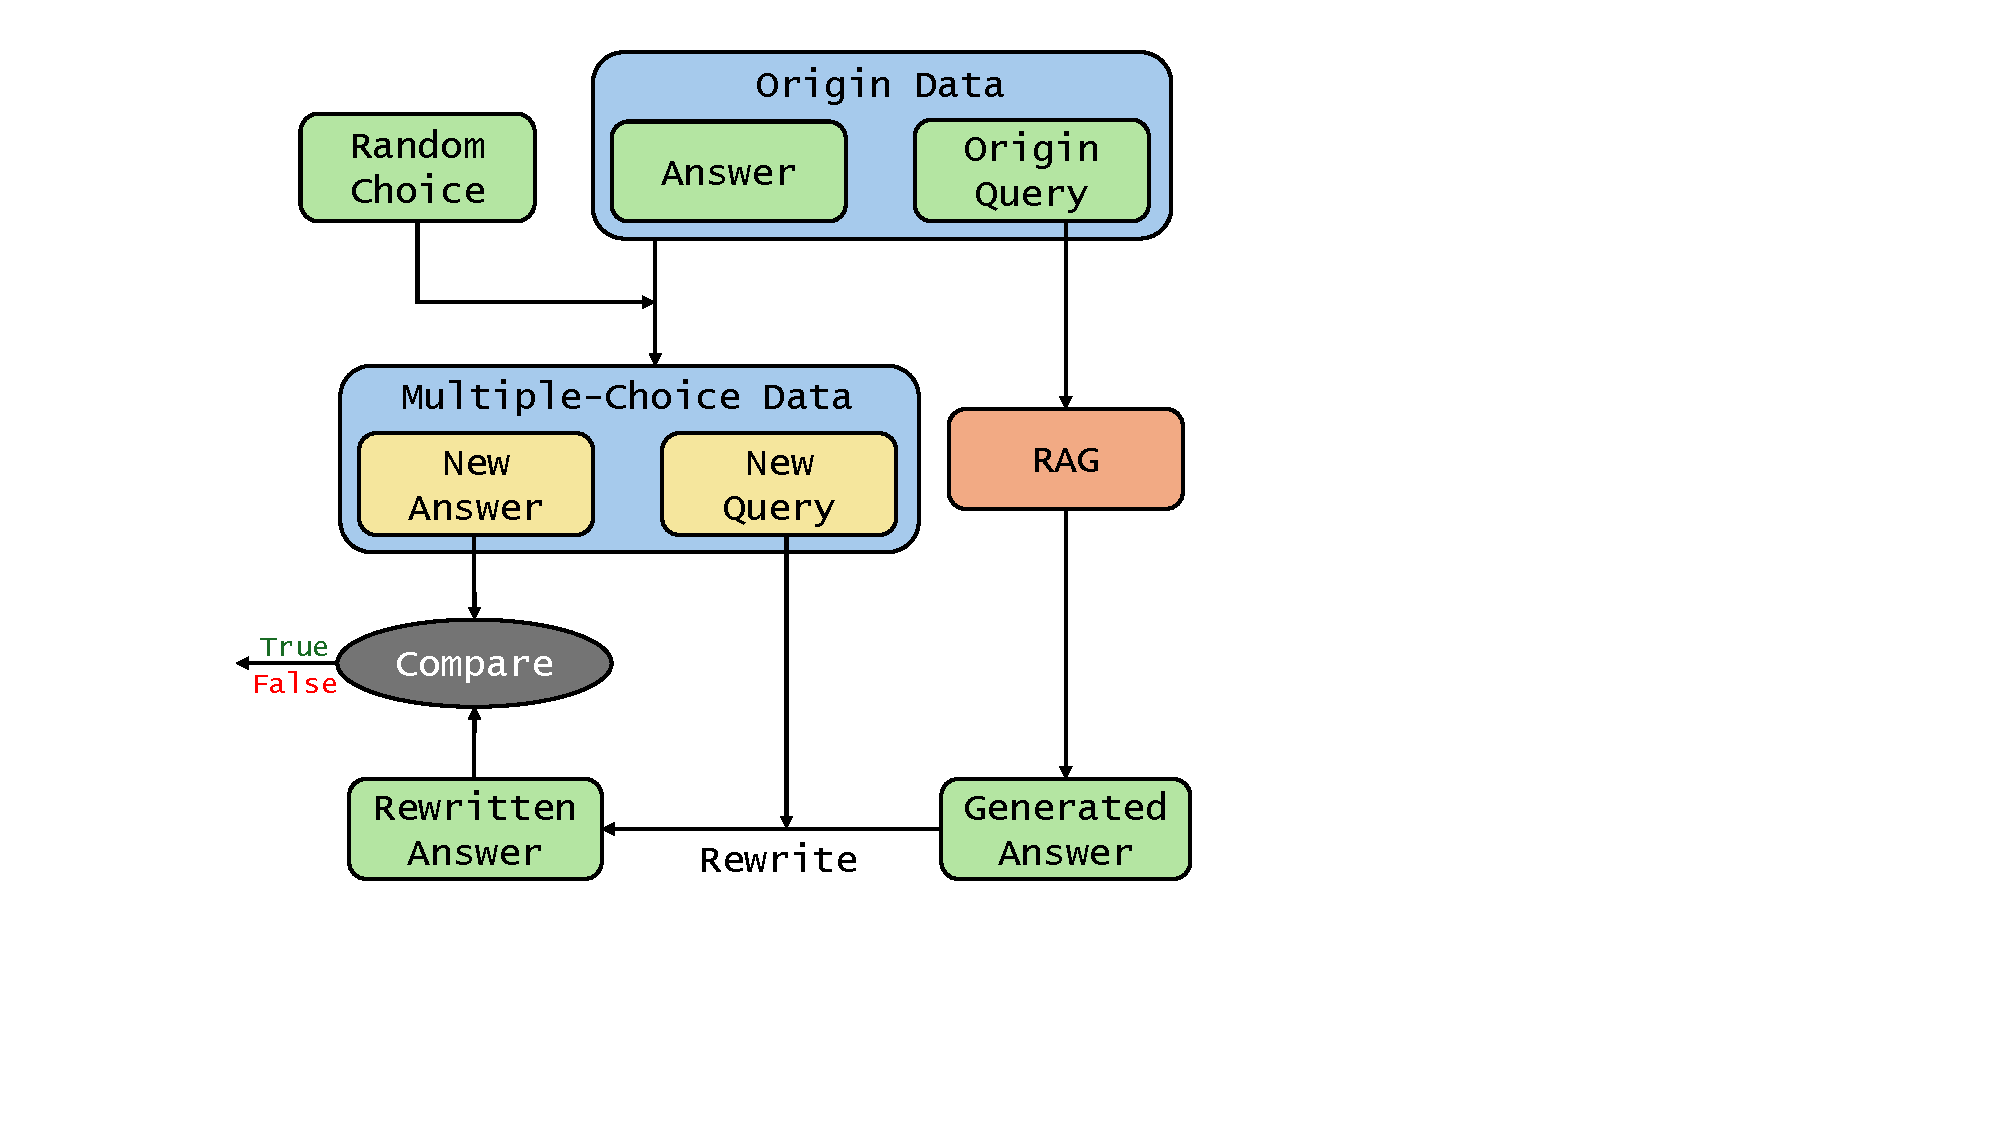
\includegraphics[width=0.5\textwidth]{Resources/LooGLE_Test_Pipeline.pdf}
    \caption{LooGLE Test Pipeline}
    \label{fig:loogle-test-pipeline}
\end{figure}

To prevent potential information leakage and ensure fair evaluation, we implement a two-stage processing strategy: First, the original question is fed into the retrieval system; subsequently, GPT-4o selects the most appropriate answer from the generated options based on the retrieval results (with the option to abstain if confidence is insufficient). The detailed prompt template for option selection is provided in \Cref{tab:option-selection-prompt}. This design maximizes the objectivity and scientific rigor of the evaluation process. Some dataset samples are illustrated in \Cref{appendix::multi-choice-loogle-dataset}. 


\subsection{Multiple-Choice Format of the LooGLE Dataset}
\label{appendix::multi-choice-loogle-dataset}

This section presents several examples from the multiple-choice version of the LooGLE dataset for reference. As shown in \Cref{fig:dataset-sample-1}, for the original question, both \ours~ and other baseline methods face challenges in evaluation because all four options are presented in a (number-number) pair format. Consequently, when verifying answers, LLMs struggle to determine whether the model's response refers to an option or the actual answer.

Additionally, as illustrated in \Cref{fig:dataset-sample-2}, we observe that nearly all methods incorporate the evidence "but is available second-hand." into their responses. However, during answer verification, the model lacks awareness of whether this information is factually correct. Since the LooGLE reference answer does not include this detail, such responses are incorrectly judged. These cases are not uncommon, which motivated our modifications to the dataset.

\begin{figure}[htbp]
    \centering
    \begin{subfigure}[b]{0.45\linewidth}
        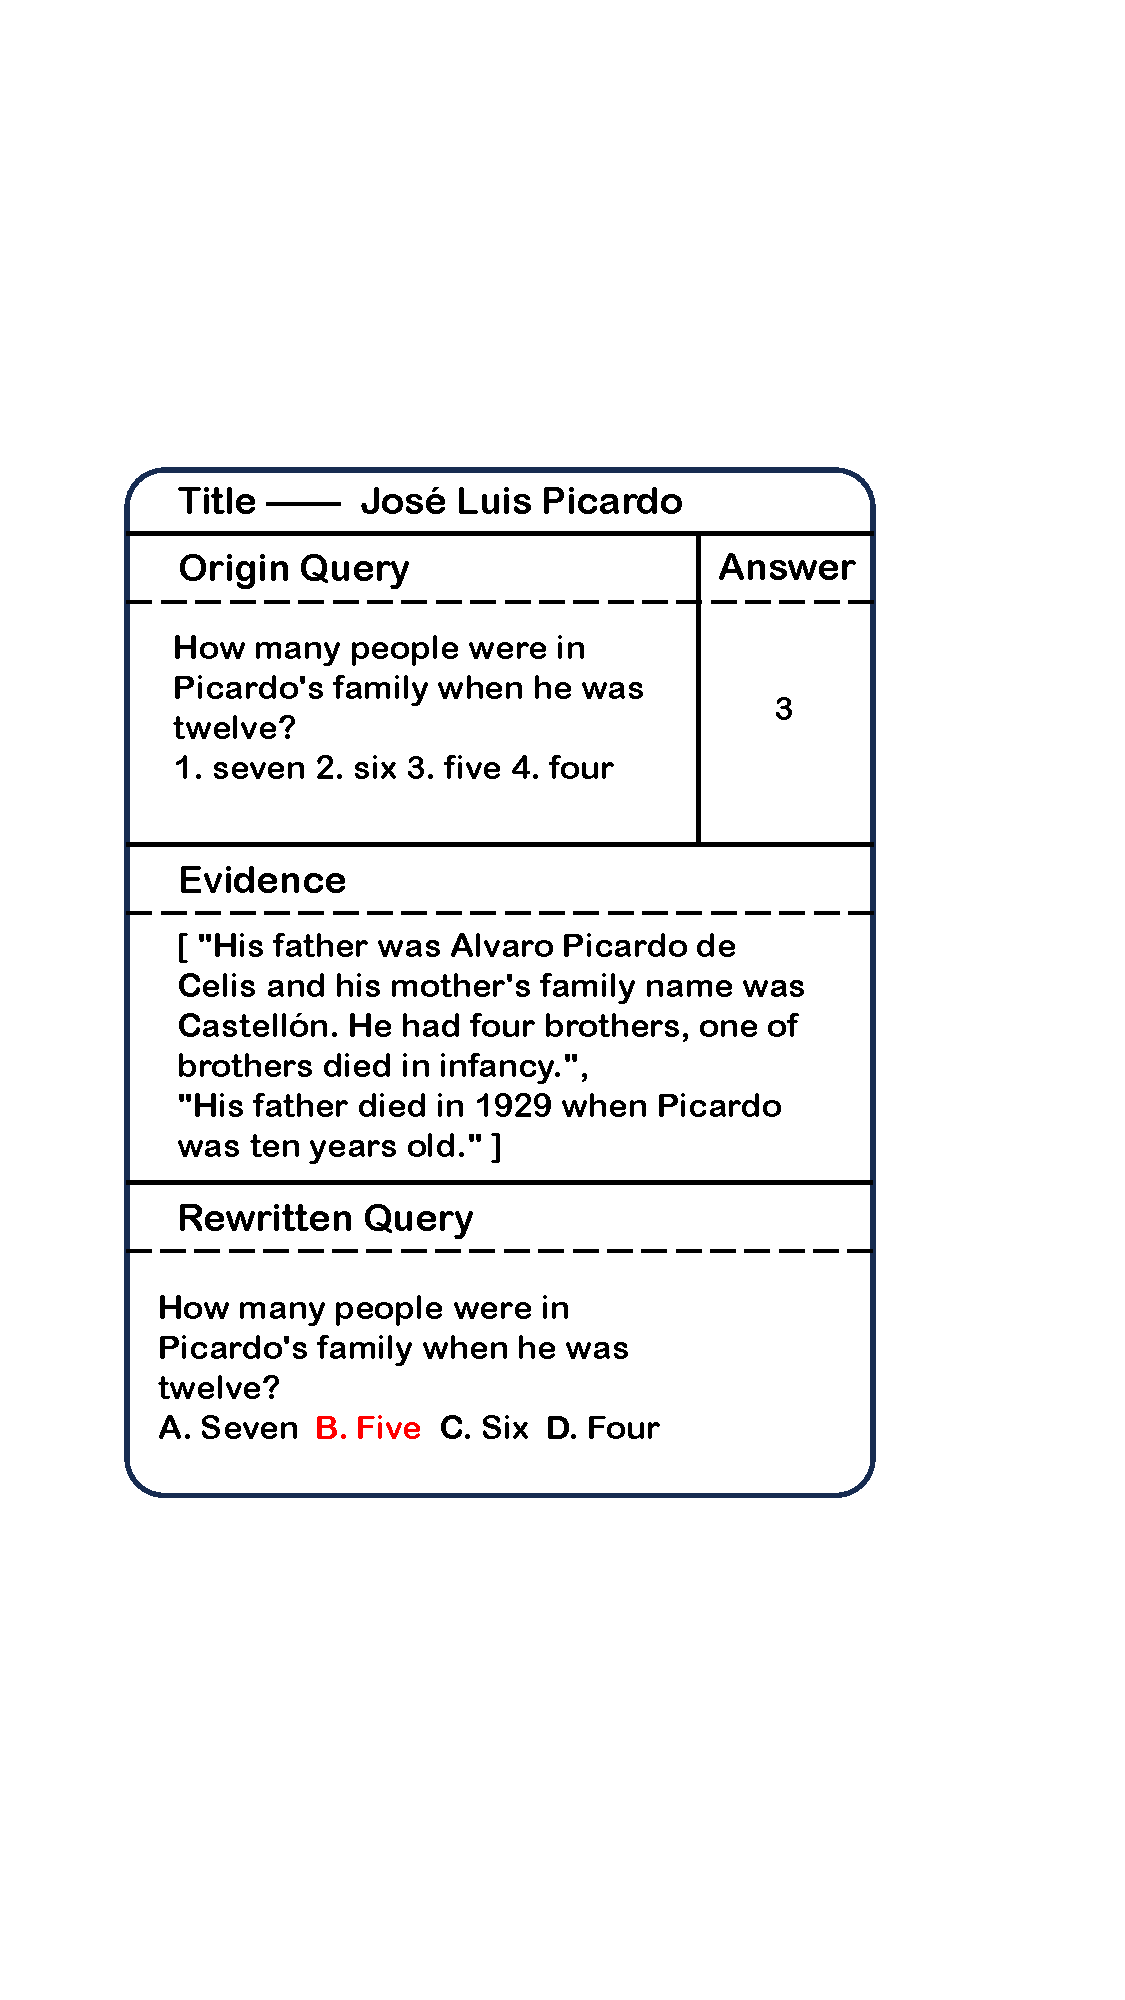
\includegraphics[width=\linewidth]{Resources/Dataset_Sample_1.pdf}
        \caption{Ambiguous Answer Reference}
        \label{fig:dataset-sample-1}
    \end{subfigure}
    \hfill
    \begin{subfigure}[b]{0.45\linewidth}
        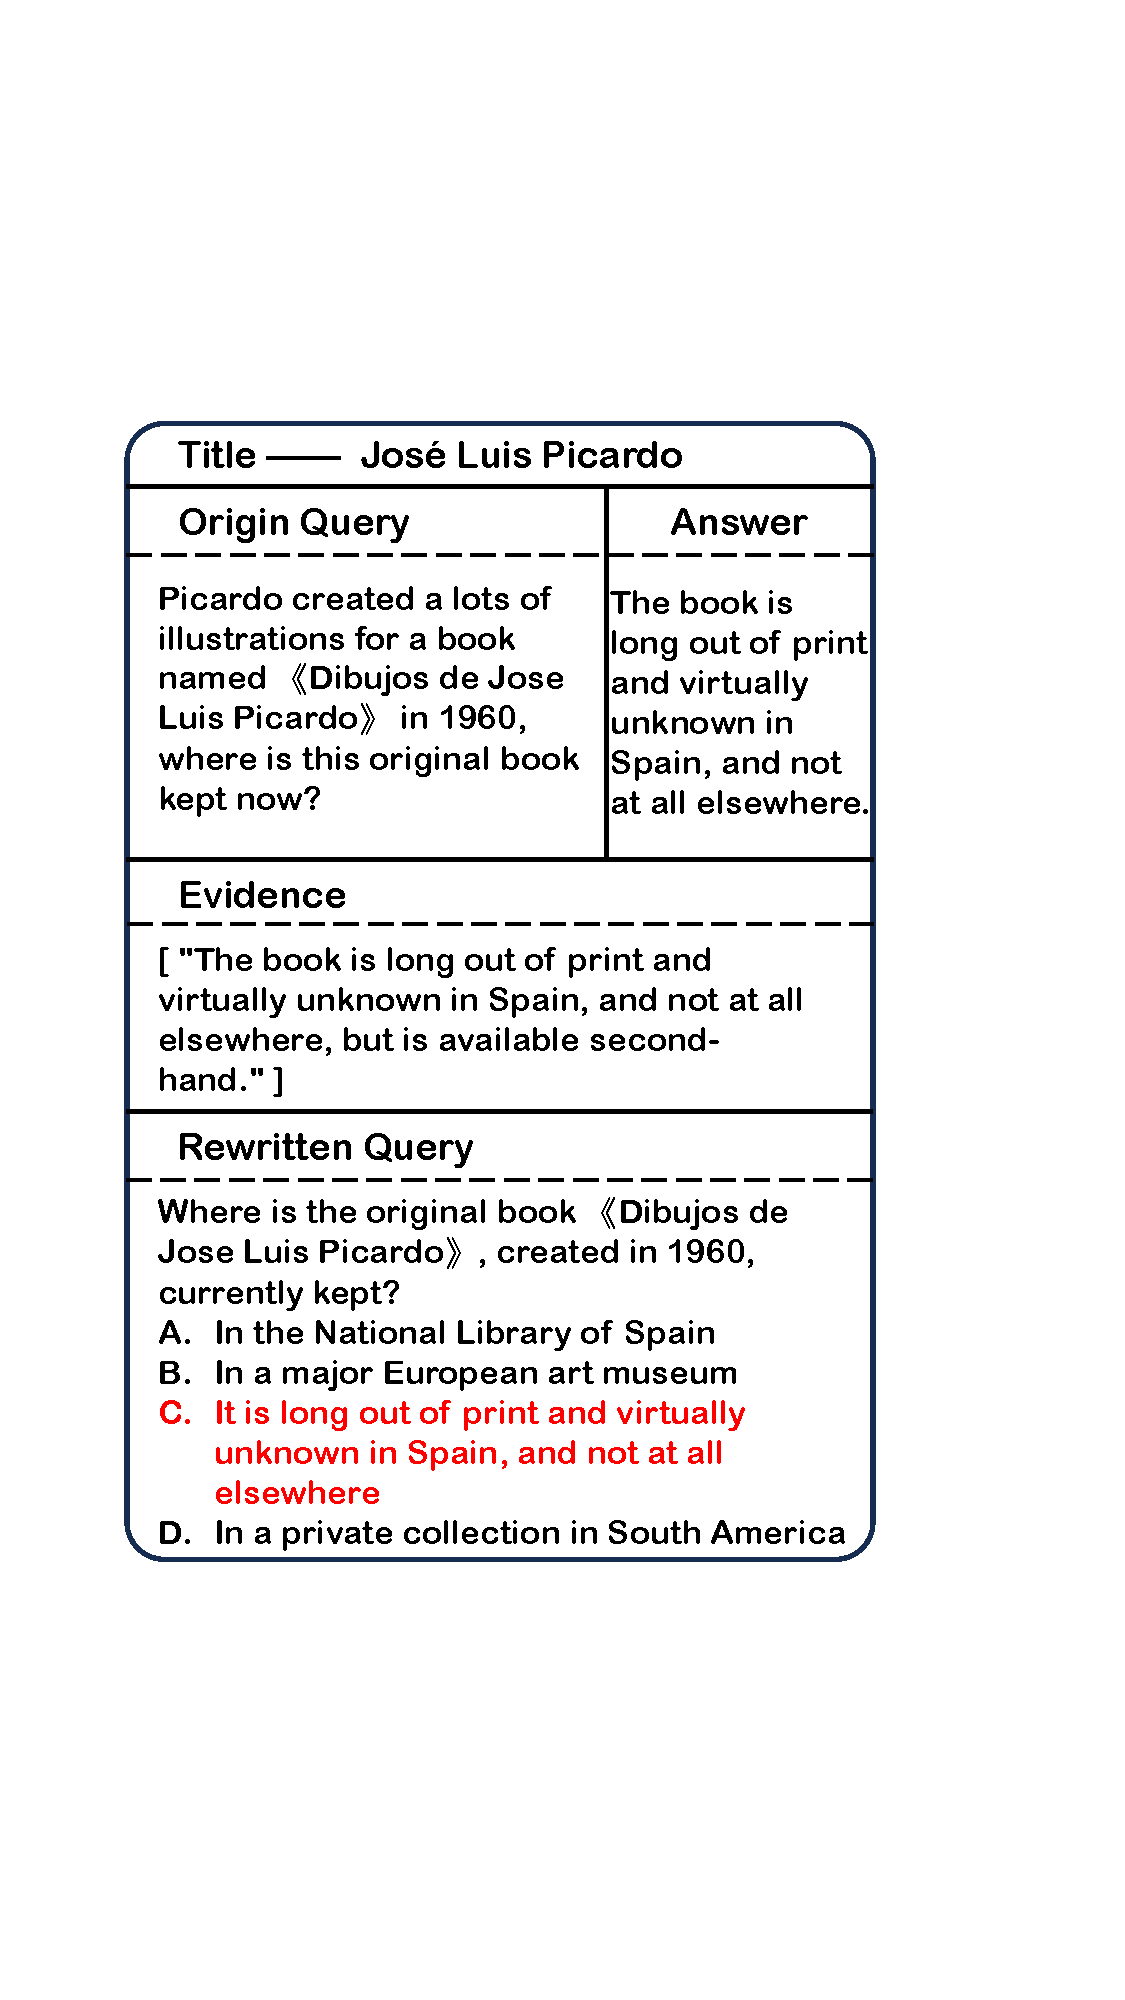
\includegraphics[width=\linewidth]{Resources/Dataset_Sample_2.pdf}
        \caption{Insufficient Answer Information}
        \label{fig:dataset-sample-2}
    \end{subfigure}
    \caption{LooGLE Dataset Samples}
    \label{fig:dataset-samples}
\end{figure}


\subsection{Similar Question Rewriting Details}
\label{appendix::similar-question-rewrite}

For questions in "Long Dependency QA" and "Hotpot QA", we employed the prompt templates from \Cref{tab:similar-rewrite-prompt} to rewrite them. While preserving the essence of each question, we aimed to maximize the surface-level differences between the rewritten and original versions. A concrete example of such rewriting is provided in \Cref{fig:similar-question-example}.

\begin{figure}
    \centering
    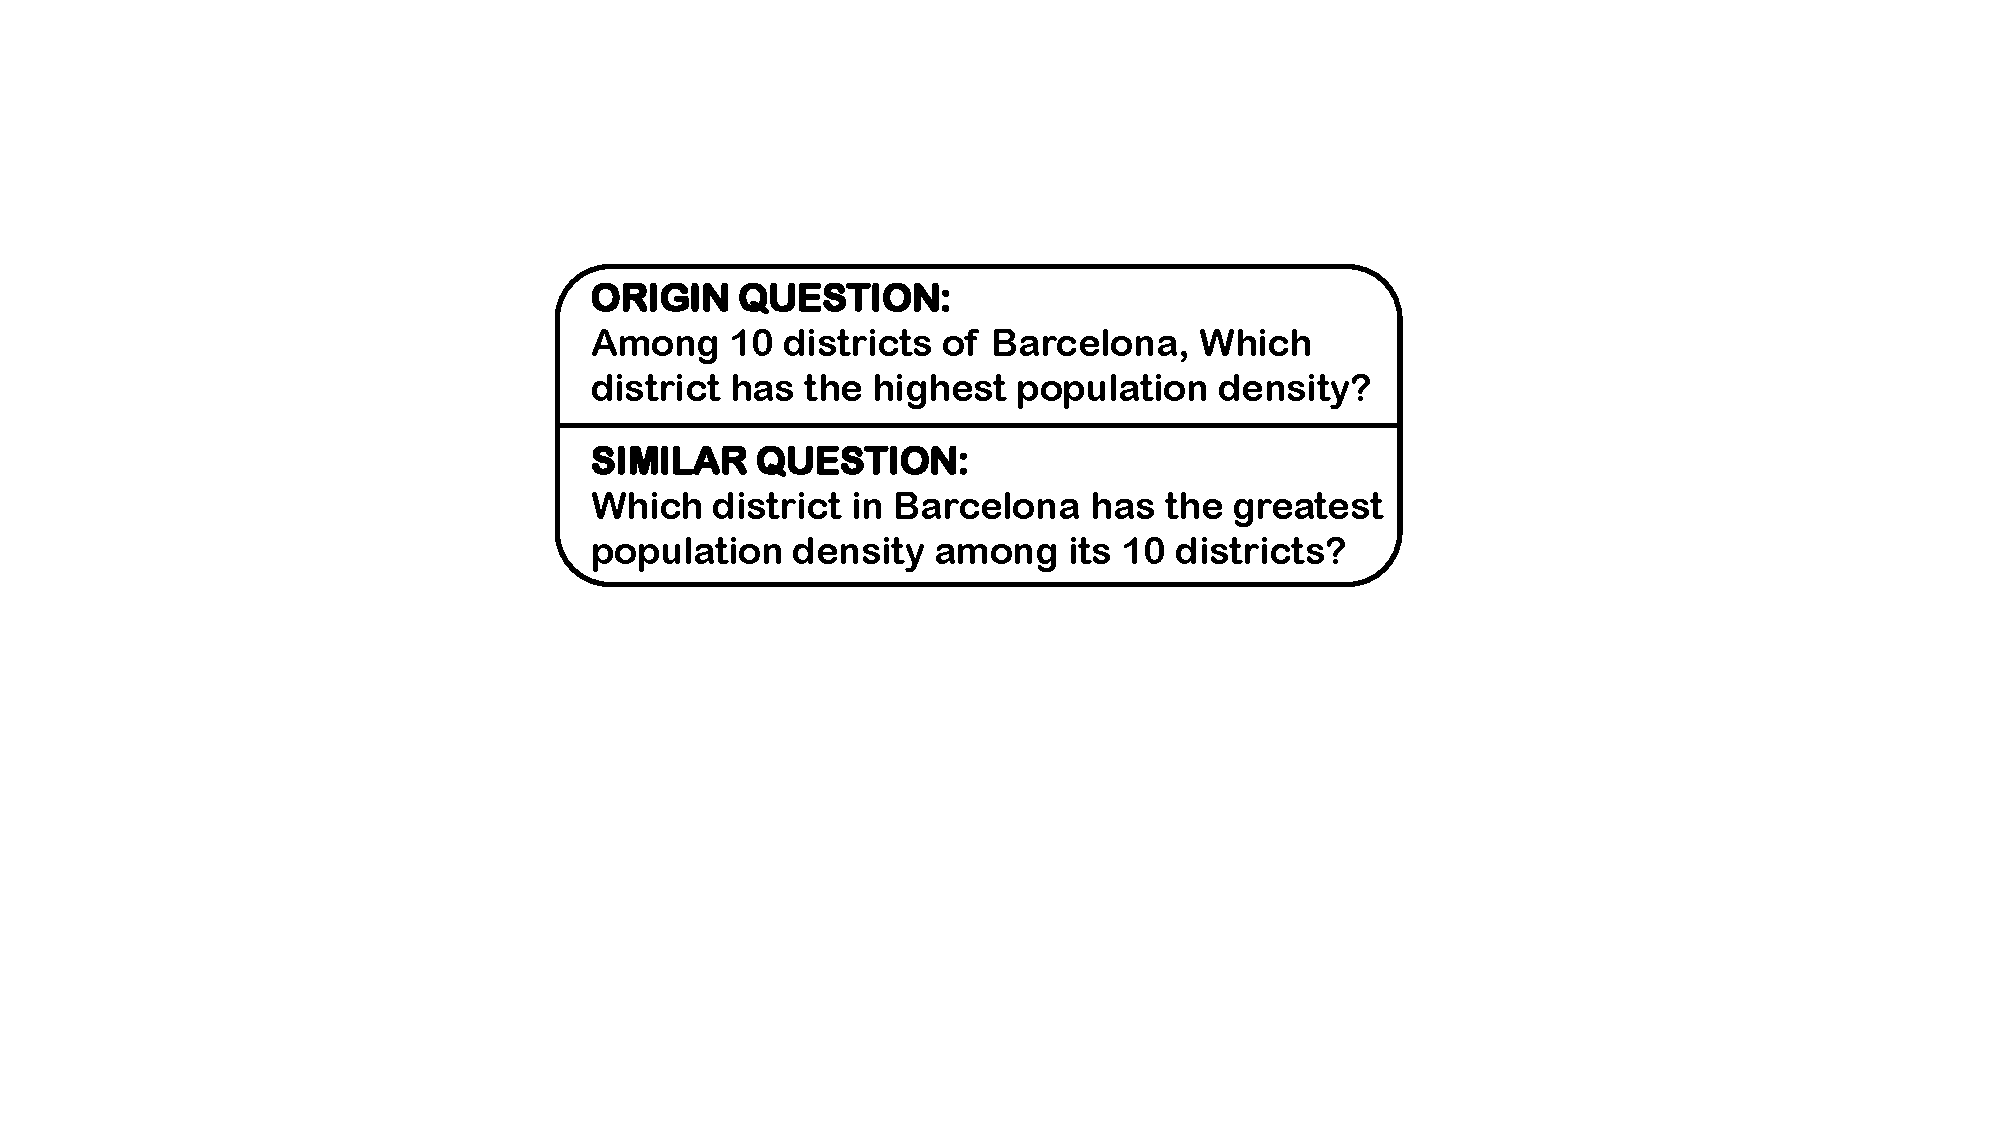
\includegraphics[width=0.5\textwidth]{Resources/Similar_Question_Sample.pdf}
    \caption{An Example of Similar Question in LooGLE}
    \label{fig:similar-question-example}
\end{figure}

\begin{figure}
    \centering
    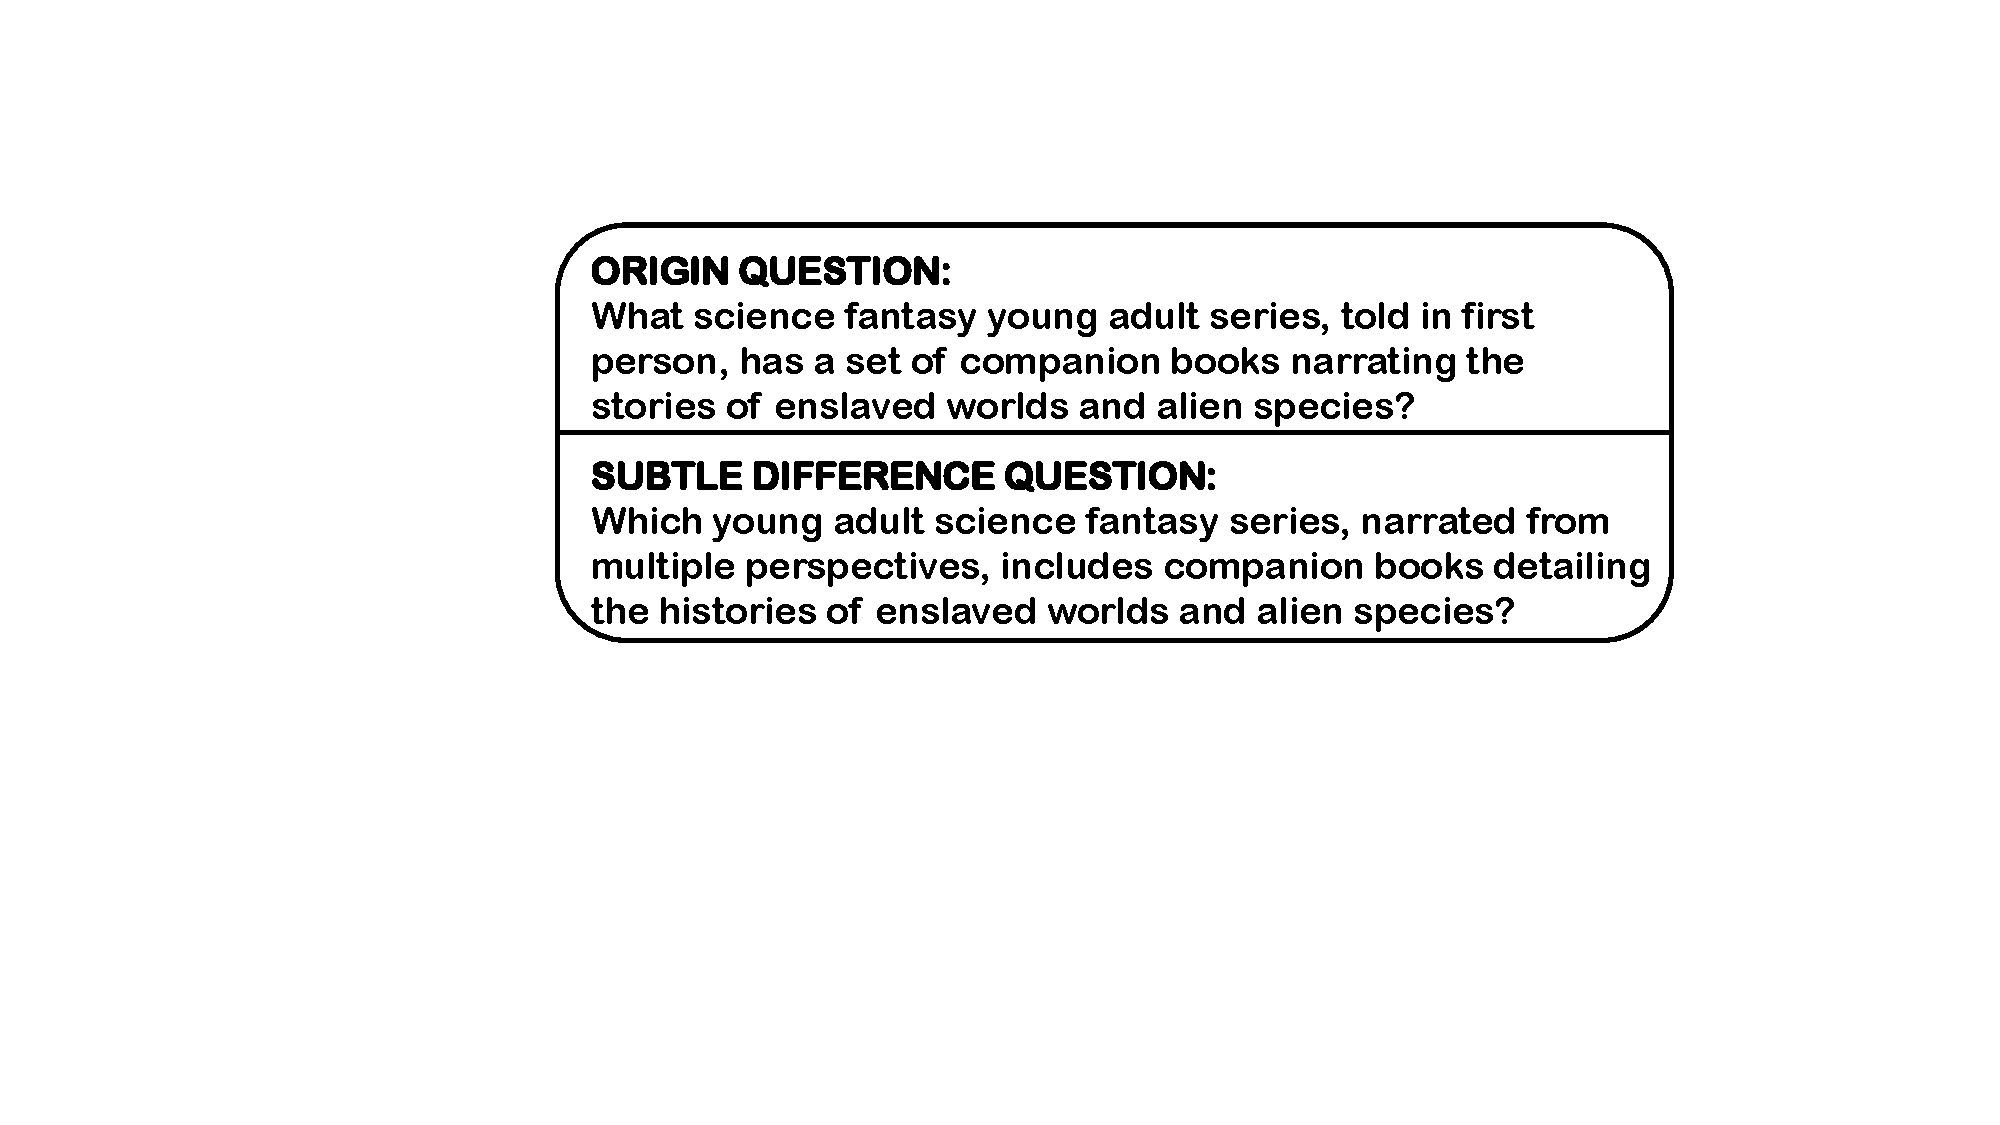
\includegraphics[width=0.63\textwidth]{Resources/Different_Question_Sample.pdf}
    \caption{An Example of Subtle Difference Question in Hotpot QA}
    \label{fig:different-question-example}
\end{figure}


\subsection{Subtle Differences Question Rewriting Details}
\label{appendix::different-question-rewrite}
For questions in "Hotpot QA", we used the prompt templates from \Cref{tab:different-rewrite-prompt} to rewrite them. While maintaining as much semantic similarity as possible, we altered the questions so that their answers differed from the original versions. A specific rewriting example is shown in \Cref{fig:different-question-example}.

